%************************************************
\chapter{Information Bottleneck and Representation Learning}\label{ch:ib_and_rl}

%************************************************
\begin{quotation}
	\small \textit{ \flushright
	We know the past, but cannot control it.\\
	We control the future, but cannot know it.
	\flushright --- Claude Shannon\\
	\vspace{1cm}}
\end{quotation}


This chapter presents the idea of using the \acf{IB} method for representation learning in general, not specific for Deep Learning, which will be the subject of \cref{ch:ib_and_dl}.

In \cref{sec:why_representation_learning}, we show \emph{why} to learn representations. In \cref{sec:desiderata}, we discuss \emph{how} to characterize a good representation. \cref{sec:2_levels} presents the two levels of representation in learning, which will help us understanding \emph{what} to represent. In \cref{sec:ib_learning}, we finally present the IB Learning concept, its difference to the IB method,  \emph{how} to find good representations with it, and its strengths and weaknesses as a representation learning framework. We close the chapter with \cref{sec:efficient_color_naming} that shows evidence that the IB framework can predict bounds on human learning.

% Thishby argues that he does not want to use the IB framework to find good representations.  His view is that the IB framework is useful to explain what happens during learning.
% The role of noise. We can control noise.



\section{Representation Learning}\label{sec:why_representation_learning}
In our human experience, we know that a good representation of data is crucial for accomplishing tasks. The Hindu-Arabic numeral system advantages, for example, are so manifest that it has been adopted almost everywhere.

In the history of Machine Learning, good representations have always played a central role. In its first years, before trying to solve a task, researchers would \emph{feature engineer}: use their knowledge of the problem in hand to \emph{encode} the data into a representation easier for computers to learn the task.

The goal of designing features is to separate explanatory factors of variation behind the high dimensional observed data. The challenge is that many of the ``factors of variation'' influence every piece of data we can observe~~\cite{goodfellow:2016}.

Consider the problem of Object Classification\footnote{\emph{``What object does this picture represent?''} Object Classification is the task of assigning a category (a label) for an image.}, each pixel depends on different factors: the viewing angle of the picture, the object's pose, the quality and calibration of the lens, the conditions of lightning, unrelated background objects, etc.

Over time, it became clear that the success of machine learning was so heavily dependent on appropriate features that finding them should also be part of the process of learning itself. Therefore, \bt{representation learning} or \bt{feature learning} is a set of techniques that allows a machine to both learn features and use them to perform a specific task.
\begin{align*}
  \underset{\text{input}}{\rvX} \xrightarrow{\hspace*{0.2cm}\text{encoder}\hspace*{0.2cm}}\underset{\text{features}}{\rvZ} \xrightarrow{\hspace*{0.2cm}\text{decoder}\hspace*{0.2cm}}\underset{\text{output}}{\hat{\rvY}}
\end{align*}
Learned representations often result in better performance and flexibility, allowing a more straightforward adaptation of an AI system to new tasks, with minimal human intervention~~\cite{goodfellow:2016}. Furthermore, the recent success of Deep Learning, which is one of many ways to learn representations, has shown the power of this \emph{encoder-decoder} scheme.

\section{Desiderata for representations}\label{sec:desiderata}
What are good representations of the data? A good representation makes a subsequent learning task easier~\cite{goodfellow:2016}.

\citeauthor{achille:2017emergence}~\cite{achille:2017emergence} present a mathematical definition using information theory.

\begin{description}[wide=0\parindent]% \setlength\itemsep{0em}\leftmargin=0pt
    \item [task]: In supervised learning, we want to find the stochastic conditional distribution \textbf{$p(y|x)$} of a target variable $\rvY$ that we refer as the \textbf{task}:
    \begin{align*}
        \rvY := P(\rvY|\rvX=x)
    \end{align*}
    \item [representation]: $\rvZ$ is a representation of $\rvX$ if it can be fully described by the stochastic conditional $p(z|x)$:
    \begin{align*}
        \rvZ := P(\rvZ|\rvX=x)
    \end{align*}
  \item[sufficient:] $\rvZ$ is a sufficient representation of $\rvX$ w.r.t $\rvY$ if $\rvY \to \rvX \to \rvZ$ form a markov chain and:
    \begin{align*}
        \IZY=\IXY.
    \end{align*}
    \item[minimal:] $\rvZ$ has the smallest amount of information among all sufficient representations of $\rvX$.  This means there is an encoding from $\rvX$ to $\rvZ$ that keep only relevant information\footnote{Minimal representations are normally equated to low-dimensional data. But, as we have exposed in \cref{ch:information}, a high dimensional representation can have little information. For example, sparse representations, that force most of its bits to be zero, are high-dimensional low-informational representations.}:
  \begin{align}
      \exists ~\rvZ~ | ~~ \IZX = \IZY = \IXY
  \end{align}
  \item[invariant:]
%   if you have a random variable that is independent to the target, your representation should also be independent to it.
to the effect of nuisances (noise)\footnote{Nuisances are factors of variation that affect data, but are otherwise irrelevant for the task.}. Let $\rvN$ be a nuisance for the task $\rvY$. If $\rvN$ does not have information about $\rvY$, there should not be information of $\rvN$ in the representation $\rvZ$ otherwise the classifier could fit to spurious correlations:\begin{align}
    \rvN\perp \rvY &\Rightarrow I[N;Y]=0 \nonumber\\
    &\Rightarrow I[Z;N]=0
  \end{align}
  \item[maximally disentangled:] information lies on components of the representation $\rvZ$ and not in the correlations of them. Mathematically, let $TC$ denote the total correlation between components of $\rvZ$~\cite{achille:2017emergence} :
  \begin{align}
    TC(\rvZ)=& \KL(p(z)||\prod_i^n p(z_i)),\\
    TC(\rvZ)=& 0 \implies z_1 ~\ind~ z_2 ~\ind~ \cdots ~\ind~ z_n.
  \end{align}
\end{description}

This desiderata for representations corresponds directly with our goals for learning algorithms. We want our models to predict the task correctly (sufficiency). Simultaneously, we want them to generalise to out-of-sample examples (invariance to nuisance factors).

\begin{figure}[hbt]
    \begin{align*}
         \text{accuracy} &\leftrightarrow \text{sufficiency}\\
         \text{generalisation} &\leftrightarrow \text{invariance/minimality}\\
         \text{explainability} &\leftrightarrow \text{disentanglement}
    \end{align*}
    \caption{Correspondence of desired properties of learning algorithms and representations.}
    \end{figure}

Another desired characteristic, albeit often forgotten, is that we want our models to be explainable\footnote{Disentanglement and minimality also simplify the subsequent inference (decoding).}. This relates to \emph{disentangling} the underlying causes (factors) of the observed data (maximally disentangled)~\cite{goodfellow:2016}.

Although disentanglement may be an abstract characteristic not very well defined,~\citeauthor{achille:2017emergence}~\cite{achille:2017emergence} propose a simplification by defining it as the total correlation of the representation features.

The only property of the desiderata that does not correspond with learning algorithms is \emph{minimality}. However, it is straightforward that a small sufficient representation has a smaller chance of containing spurious correlations, and it is more likely to generalise well.  Minimal sufficient representations have no spurious factors that do not explain the variability of the observed data.  As we will show, a representation is invariant only if it is also minimal.

\subsection{Invariant if minimal}\label{sec:invariant_if_minimal}

\begin{theorem}[\citeauthoritle{achille:2019phd}\cite{achille:2019phd}, Proposition 2.4.1] Let $\rvN$ be a nuisance for the target $\rvY$ and let $\rvZ$ be a sufficient representation of the input $\rvX$ w.r.t $\rvY$. Suppose that $\rvZ$ depends on $\rvN$ only through $\rvX$ ( i.e.\ , $\rvN \to \rvX \to \rvZ$). We also consider that $\rvX$ has all information about $\rvY$, therefore we can say that it is a deterministic function of $\rvY$ and nuisances $\rvX:= f(\rvY; \rvN)$.

To say that   $\rvZ$ is invariant if and only if it is minimal implies that $\IZN = \IZX - \IXY$:
\begin{align*}
    \forall~ \rvZ ~|~ \IZY = \IXY, \nonumber\\
    \IZX = \IXY \Longleftrightarrow \IZN = 0, \nonumber\\
    \IZN = \IZX - \IXY.
\end{align*}
This equality holds up to a small residual $\epsilon$:
\begin{align}
	\IZN &= \IZX - \IXY - \epsilon,	~0 \leq \epsilon \leq H[\rvY|\rvX]
\end{align}

\end{theorem}
\begin{proof}
	\begin{align*}
    \begin{cases}
    \rvY, \rvN \to \rvX \to \rvZ \qquad &\text{(hypothesis)}\\
    I[\rvZ;\rvY,\rvN] \leq I[\rvZ;\rvX] \qquad &\text{(DPI)}\\
    I[\rvZ;\rvY,\rvN] = I[\rvZ;\rvN] + I[\rvZ;\rvY|\rvN] \qquad &\text{(chain rule)}
    \end{cases}
    \end{align*}
    \begin{align}
    &I[\rvZ;\rvN] + \cancelto{\scriptscriptstyle \IZY}{I[\rvZ;\rvY|\rvN]} \leq I[\rvZ;\rvX] \tag{$\rvN \ind \rvY$}\\
    &I[\rvZ;\rvN] \leq I[\rvZ;\rvX] - \cancelto{\scriptscriptstyle \IXY}{\IZY} \tag{$\rvZ$ sufficiency}\\
    &I[\rvZ;\rvN] = I[\rvZ;\rvX] - \IXY -\epsilon, \epsilon \geq 0 \tag{missing $\epsilon$ upperbound}
    \end{align}
Now we only need to prove the upperbound for $\epsilon$:
\begin{align}
    \epsilon &= \IZX - I[\rvZ;\rvN] - \IXY \nonumber\\
     &= I[\rvZ;\rvY,\rvN] - I[\rvZ;\rvN] - \IXY \tag{$\rvX:=f(\rvY; \rvN)$}\\
     &= \cancel{I[\rvZ;\rvN]} + I[\rvZ;\rvY|\rvN] - \cancel{I[\rvZ;\rvN]}- \IXY \tag{chain rule}\\
     &= \cancelto{\scriptscriptstyle H[\rvY]}{H[\rvY|\rvN]} - H[\rvY|\rvN;\rvZ] - H[\rvY] + H[\rvY|\rvX] \tag{$\rvN \ind \rvY$}\\
     &= \cancel{H[\rvY]} - H[\rvY|\rvN;\rvZ] - \cancel{H[\rvY]} + H[\rvY|\rvX] \nonumber\\
     &\leq  H[\rvY|\rvX] \tag{$\epsilon$ upperbound}
\end{align}

$I[\rvZ;\rvN] = I[\rvZ;\rvX] - \IXY -\epsilon, ~0 \leq \epsilon \leq H[\rvY|\rvX]$\end{proof}

As a consequence of this proposition, it is possible to construct invariant representations, which will generalise well, by reducing the amount of information the representation $\rvZ$ contains about the input $\rvX$ while keeping $\IZY$, the amount of information we need for the task. As $H[\rvY] \ll H[\rvX]$~\textbf{generalisation is determined by the compressibility of the input}. Thus, it is independent on the hypothesis space of the learning algorithm.

\section[IBT Learning Problem]{IBT Learning Problem: Learning Approximately Minimal Sufficient Disentangled Representations}\label{sec:ibt_learning_problem}}
    We have discussed what consistitute a good representation. This section is about finding them. For that, we will adjust the IB Problem Setting (\cref{ib_problem_setting}) for supervised learning\footnote{Trying to be consistent with \cref{ch:mlt, ch:ib}, we will repeat some definitions in this section.}.
    \begin{figure}
      \centering
         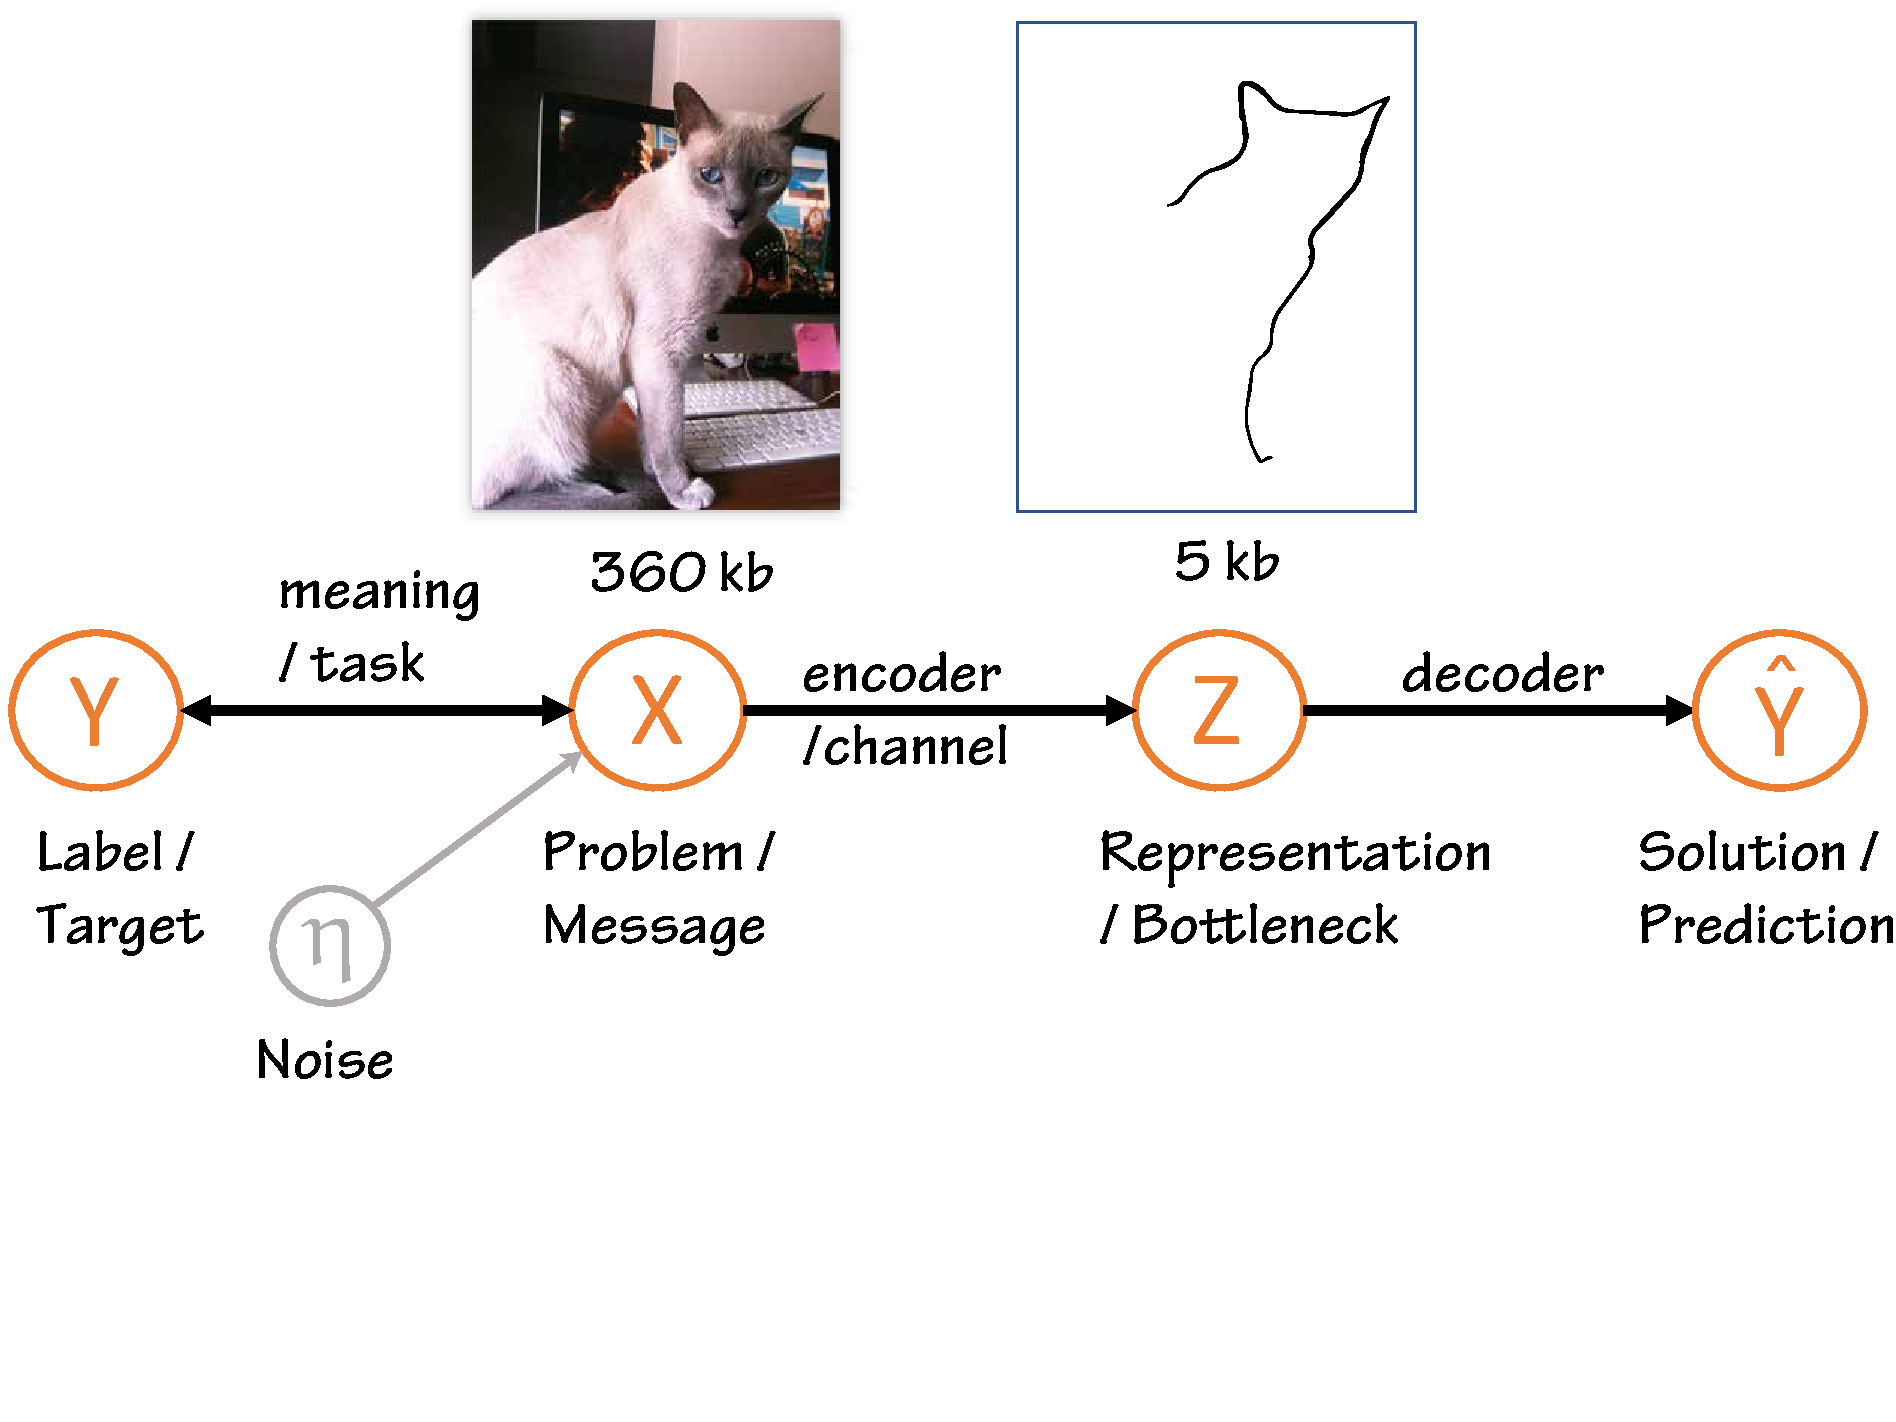
\includegraphics[width=1\linewidth]{ibt_learning_problem}
         \caption{The \ac{IBT} Learning Problem is the adaptation of the IB Problem to the learning setting.}
         \label{fig:ibt_learning_problem}
      \end{figure}

    \subsection{Definitions}
    \begin{enumerate}
      \item Let $\rvX$ be the random variable that denotes the
       \textbf{generator} (or \textbf{source}) of instance vectors $\rx$ of the learning problem  (\textbf{messages}), randomly draw from a probability distribution \(P(\rvX)\),\\ \(x\sim P(\rvX),~ x \in \sA_{\rvX} \);
       \item Let $\rvY$ be a random \textbf{relevant variable}  (the \textbf{Target}) which represents the solution $\ry$ for the problem $\rx$,~\ie the intended meaning $p(y|x)$ of the message $x$,\\
       \(y\sim P(\rvY),~ y \in \sA_{\rvY} \);
      \item A \textbf{task supervisor} knows the \textbf{task} distribution $P(\rvY|\rvX)$ and returns an output vector \(\ry_i\) for every input vector \(\rx_i\):\\
      $y_i := p(y|x_i)$;
      \item Let $\rvZ$ be a \textbf{bottleneck} random variable that denotes a compressed representation of the input $\rvX$ that is sufficient w.r.t. $\rvY$ and obeys the Markov chain $\rvY \leftrightarrow \rvX \leftrightarrow \rvZ$;
      \item Let the stochastic conditional distribution $q(z|x)$ be an \textbf{encoder}\footnote{A lossy encoder can be seen as a noisy channel.}of input instances into representations,\\
      $\rz := q(z|x)$.
      \item Let the stochastic conditional distribution $q(y|z)$ be a \textbf{decoder} of representations into solutions of the problem,\\
      $\hat{\ry} := q(y|z)$.
      \item A \textbf{learning algorithm} \(\AA\) which is the functional that given a dataset \(D_n = \{(\rx_1,\ry_1), \cdots, (\rx_n, \ry_n)\}\) of $n$ inputs and outputs of the task, selects a hypothesis \(h = \underset{\text{decoder}}{q(y|z)} \circ \underset{\text{encoder}}{q(z|x)} \) from the hypothesis space \(\HH\):
      \begin{align}
        \AA: \underbrace{(\XX \times \YY)^n}_{D_n} \to \HH .
      \end{align}
    \end{enumerate}

  \subsection{Assumptions}\label{sec:ibt_learning_assumptions}
  \begin{enumerate}
    [i.]
    \item The random variables $\rvX$, $\rvY$ and $\rvZ$ are \textbf{discrete};
    \item $\rvY \to \rvX \to \rvZ$ form a Markov-chain;
    \item $\sA_{\rvX}$, $\sA_{\rvY}$ and $\sA_{\rvZ}$ are \textbf{finite sets};
    \item \textbf{No assumption on \(\DD=\PXY\)}.
    \item \textbf{\(\DD=\PXY\) is unknown at the training stage}.
    \item \textbf{\(\DD=\PXY\) is fixed:} the ordering of examples in the sample is irrelevant.
    \item The generator/source $\rvX$ is an ergodic process (see \cref{ib_problem_setting}), therefore $x \sim p(x)$ are not necessarily mutually independent\footnote{This assumption is less constrained than independent sampling}.
		\item The encoder and the decoder are \textbf{stochastic} mappings \footnote{Notice that given the Markov chain $\rvY \leftrightarrow \rvX \leftrightarrow \rvZ$, due to reparemetrization invariance (Theorem \ref{th:reparemetrisation_invariance}), a deterministic mapping of the data does not throw out information, i.e. \ let $f:\aXX \to \aYY$ be deterministic, $I[f(\rvX);\rvY]=\IXY$.}.
		\item the \textbf{distortion measure} between $\rvX$ and its representation $\rvZ$ is $\IXY - \IZY = \KL(p(y|x)||p(y|z))$\footnote{This assumption is not strictly required, as it can be derived. The only reason to keep it here is to make the comparison of different problem settings easier.}.
  \end{enumerate}
\subsection{Problem statement}
Given the problem setting above, the \ac{IBT} learning problem is to find the encoder $p(z|x)$ and decoder $p(y|z)$ such that:
\begin{enumerate}
  \item the encoder maximises the compression of the input $\rvX$ into the representation $\rvZ$ while preserving the maximum information about the ``meaning'' $\rvY$. In other words, the encoder that generates minimal sufficient disentangled representations of the input.
  \item the decoder is trivial, as a result of the characteristics of the representation.
  \item The selection is based on a training set of $n$ i.i.d. observations drawn from an ergodic process $\PXY$.
\end{enumerate}
\subsection{Comparing IBT with other problems}
\subsection{IBT learning as a variational problem}
    Finding the encoder for minimal sufficient disentangled representations is equivalent to finding a distribution $p(z|x)$ that solves the following constrained optimisation problem.
    \begin{align}
        q(z|x):=\underset{p(z|x)}{\argmin} \quad  & \IZX  \\
        \textrm{s.t.}\quad
        & 0 \leq \IXY - \IZY \nonumber\\
        \quad & 0 \leq TC(Z)\nonumber
    \end{align}
    This non-linearly constrained optimisation problem\footnote{Prior to the publishing of \cite{alemi:2016} in 2017, there was no known algorithm to minimise the IB Lagrangian for discrete $\rvX$ and $\rvY$ with large state spaces or non Gaussian continuous joint distribution.} is very similar to the IB Problem (\cref{sec:IB_principle}). It just adds the total correlation constraint and assumes no knowledge over $\PXY$. ~\citeauthor{tishby:1999}~\cite{tishby:1999} proposed solving the IB problem using a relaxed minimization, the IB Lagrangian:
    \begin{equation}
        \begin{split}
        \underset{p(z|x)}{\min} \quad  & \IZX  \\
        \textrm{s.t.}\quad & \IZY \leq \IXY \\
        \end{split}
        \quad \Longrightarrow \quad
        \begin{split}
            &\min \IZX + \beta (\cancel{\IXY} - \IZY),\\
            &\min \IZX - \beta \IZY.
        \end{split}
    \end{equation}

    Let us also apply a Lagrangian relaxation to our representation learning problem:
    \begin{align}
        \LH &=  \IZX + \beta (\IXY - \IZY) + \gamma TC(z),\\
        \text{Let }\beta'&= \frac{1}{\beta}, \gamma'= \frac{\gamma}{\beta}\\
        \LH &=  \cancelto{\scriptscriptstyle \HYZ}{(\IXY - \IZY)} + \beta' \IZX + \gamma' TC(z),\\
        \LH &=  \HYZ + \beta' \IZX + \gamma' TC(z).
    \end{align}
    Let us denote $q_\theta(z|x)$ (encoder) and $q_\theta(y|z)$ (decoder) the unknown conditional distributions we want to estimate\footnote{$q_\theta(y|x)=\sum q_\theta(z|x) q_\theta(y|z)\\q(y|x,\theta^*)=p(y|x)$
    }, parametrized by $\theta$.

    Rewriting the Lagrangian as a per sample loss function, we have:
    \begin{align}
        H[\rvY|\rvZ] & \approx \E_{(x,y) \sim p(x,y)}[\E_{z \sim q_{\theta}(z|x)} - \log q_{\theta}(y|z)] \\
        \IZX & = \E_{x \sim p(x)} \KL(q_{\theta}(z|x)||p(z))\\
        TC(z) &= \KL(p(z)||\textstyle \prod_j q(z_j))\\
        \hat{\LH} &= \frac{1}{n} \sum^{n} \E_{z \sim q_{\theta}(z|x_i)} - \log q_{\theta}(y_i|z) \nonumber\\
         &+ \beta' \KL(q_{\theta}(z|x_i)||p(z)) \nonumber\\
         &+ \gamma' \KL(p(z)||\textstyle \prod_j q_{\theta}(z_j)).
    \end{align}

    The second and third terms of the loss are intractable, as we need to know $p(z)$ to compute, which is an unknown of our problem.~\cite{achille:2018infodropout}, however, prove that if $\gamma'=\beta'$, \ie we assume a factorised unknown distribution, the Lagrangian can be solved.

    \begin{align}
    \hat{\LH} = &\underbrace{\frac{1}{n} \sum^{n} \E_{q_{\theta}(z|x_i)} - \log q_{\theta}(y_i|z)}_{\hat H(p, p_{\theta})}\nonumber\\
    &+ \beta' \KL (q_{\theta}(z|x_i)||q_{\theta}(z)),~
    q_\theta(z)=\prod_j q_{\theta}(z_j).
    \end{align}

    Where $\hat H(p, p_{\theta})$ is the cross-entropy, and the second term is a regulariser that penalises the transfer of information from $\rvX$ to $\rvZ$. In other words, the regulariser penalises complexity measured as $\IZX$. The usage of cross-entropy loss and this kind of regularisers is widespread in practice. \cite{achille:2019phd} gave theoretical ground for such choices\footnote{The reference constraint their findings to \acp{DNN} optimised with \ac{SGD}. We find the result more general than that.}.

    \begin{corollary}
    Any learning algorithm that\footnote{This insight allowed \cite{alemi:2016,achille:2018infodropout} independently develop basically the same algorithm for estimating mutual information for any distribution using \acp{DNN}.}:
     \begin{itemize}
         \item assumes a stochastic $p(y|x)$;
         \item uses the cross-entropy loss;
         \item and a regularisation term that penalises the amount of information of the input stored in the model,
     \end{itemize} is learning a minimal sufficient disentangled representation and, in fact, solving a special case of the IB problem.
\end{corollary}

\section{Two levels of representation}\label{sec:2_levels}
Some criticism on works in what we are calling \emph{Information Bottleneck Theory} derive from a lack of rigour in explaining some basics (see \cref{sec:criticism}).

In \cref{ch:mlt}, we were presented with the \emph{learning problem} setting:
\begin{figure}[ht] \centering
    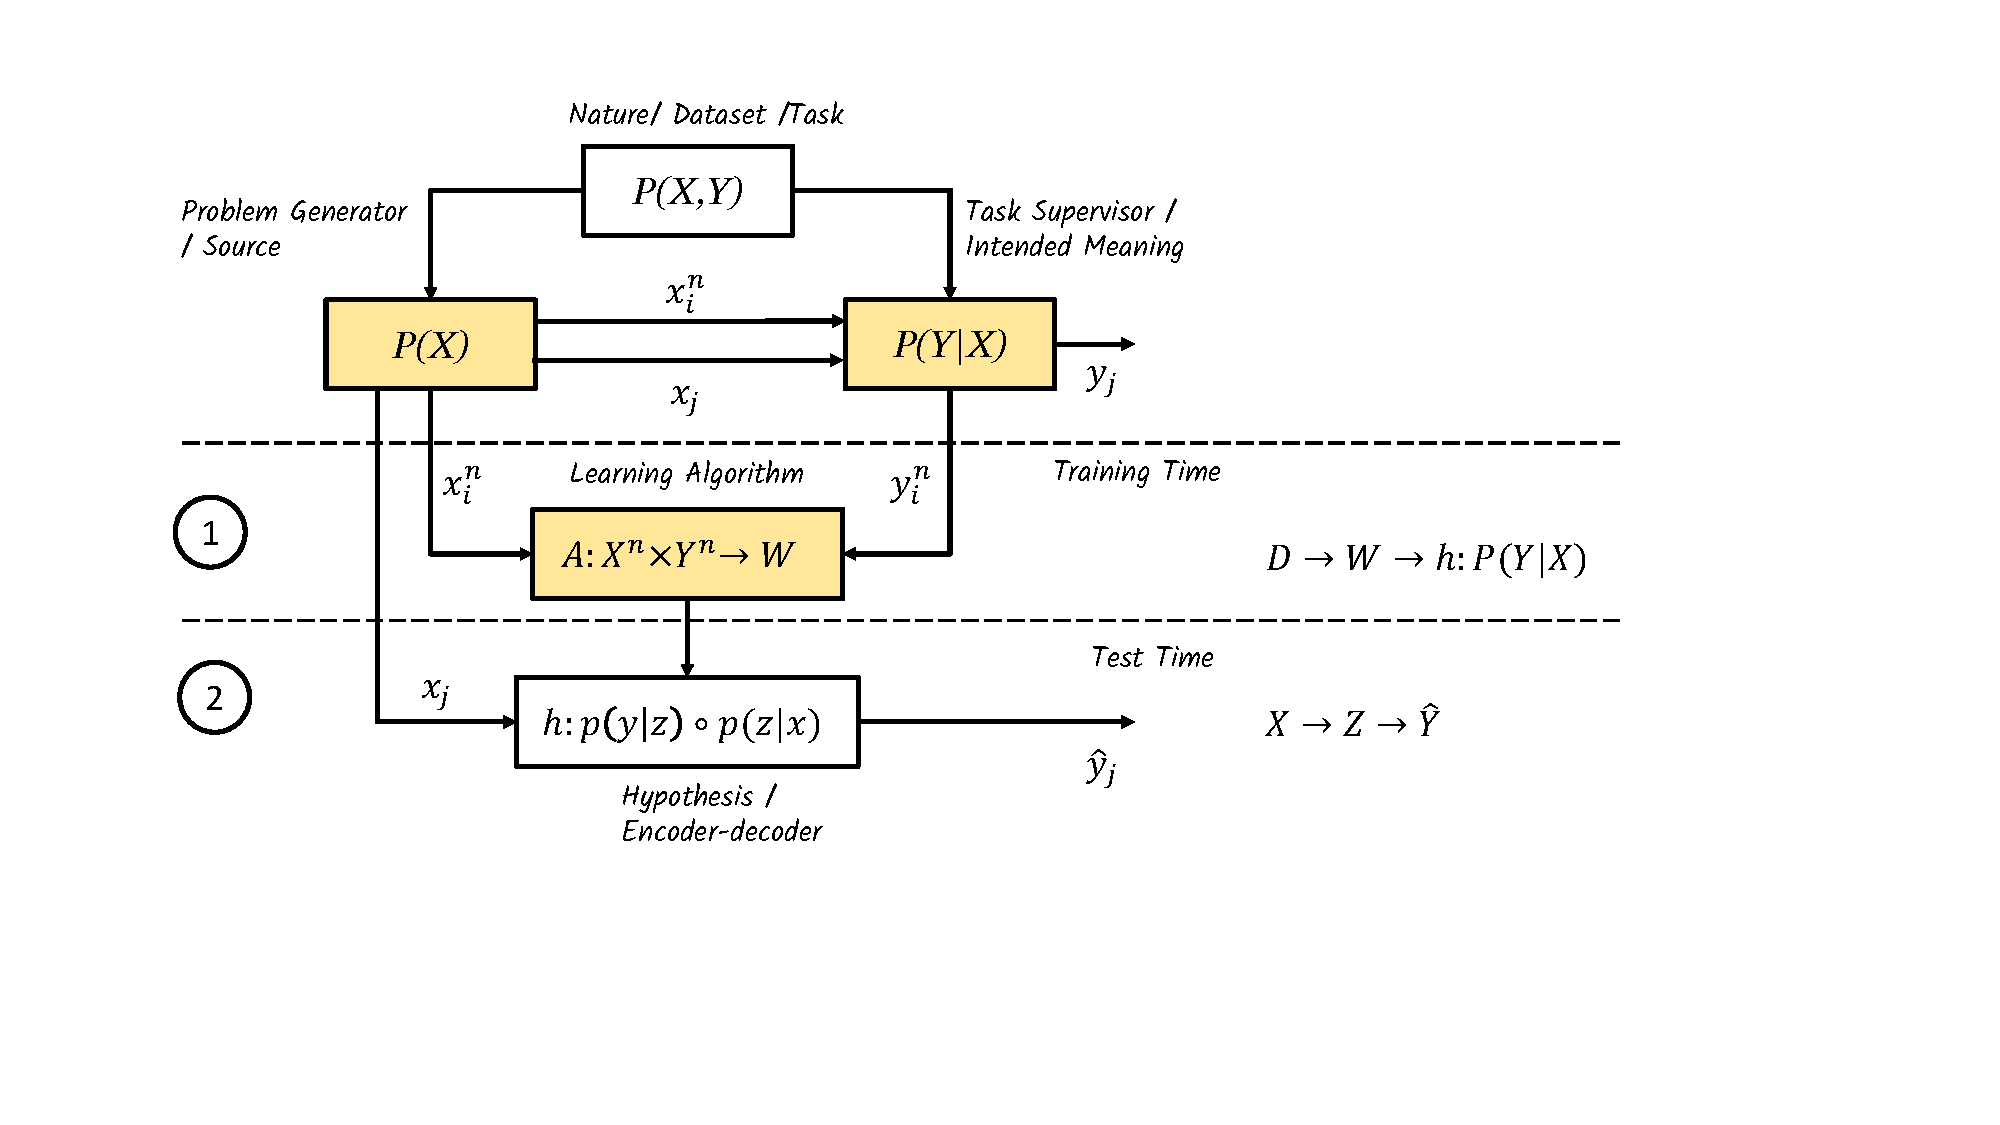
\includegraphics[width=
    \textwidth]{ibt_learning_setting}
    \caption{Two levels of representation in the learning setting.}\label{fig:two_levels_representation}
\end{figure}

The crucial problem in \ac*{MLT} is that we want to predict the behaviour (bound) of learning algorithms in future data while we can only access past performance. This dichotomy translates to representation learning by two intertwined but different representations:
\begin{enumerate}[label=\protect\circled{\arabic*}]
  \item the representation of a \emph{dataset} (past data), a function that can be stored in memory for the later accomplishment of the task. It needs to keep useful information for future decisions without squandering resources in remembering spurious correlations or one-time events.
  \item the representation of an \emph{input example} (current data): which need to keep the essence of the scene at hand;
\end{enumerate}
% Why is this important? mTishby vs Achille

In~\cite{achille:2019phd, achille:2019weights}, borrowing the terminology of Deep Learning,~\citeauthor{achille:2019phd} call these two levels of representation of \emph{information in the weights} and \emph{information in the activations}, respectively.

Several \ac{IBT} papers to not address this difference. In special, some of the seminal work \cite{tishby:2015, shwartz-ziv:2017, tishby:2017}. How can we minimise the information in the activations, while we cannot access future data? There is a missing step.

We have to show how to bound future behaviour performance based only in the available training data.

Intuitively, there is a strong connection between  \emph{information in the weights} and \emph{information in the activations}. $\IZX$ which  measures the complexity of the activations representation, can be defined by the amount of weight in the network: low or zero weights will connect to the activations that are not in the optimal activation representation $z^*$ which minimizes $\IZX$.

In \cref{sec:duality}, we will formally address this issue.

\subsection[Rethinking generalisation: \\Cross-entropy and overfitting]{Rethinking generalisation: Cross-entropy and overfitting}
 In previous sections, we derived the use of the cross-entropy loss from a list of desired properties for representations(\cref{sec:desiderata})and that generalisation relates to the compressibility of the input(\cref{sec:invariant_if_minimal}). Still, what prevents the model to only memorise the map of training examples index to labels? Such memorisation seems a valid compression, need little information and will, obviously,not generalise.

 \cite{zhang:2016} demonstrates that the expressivity of \acp{DNN} is enough to fit random labels. Thus, at least for \acp{DNN}, generalisation is more \emph{not overfitting} than {not underfitting}.  This may be the case for other learning techniques as well. In this section, we will keep \emph{rethinking} generalisation on this new information-theorethic perspective and tray to elucidate how cross-entropy loss relates to overfitting and memorisation.

Classical \ac{MLT} assumes that we select an hypothesis $h$ parametrized by $\theta$. Conceptually, we already \emph{rethought} generalisation as being determined by the compressibility of the input (\cref{sec:invariant_if_minimal}). In this sense, the task is determined by the training dataset only\footnote{\cite{achille:2019phd} defines the task as the dataset distribution for which we only have one sample.}. Thus, we will assume the dataset is sampled from some generative model $P(\rvD|\theta)$. In this context~\cite{achille:2017emergence}:
\begin{theorem}
  Given $\rvD=(\rvX,\rvY),~ \rvD \sim P(\rvX, \rvY| \theta)$, and a representation $\rvW$ of $\theta$, s.t. $\rvY|\rvX \to W \to \theta$ form a Markov-chain:
  \begin{align*}
    H_{p,q}[\rvD|\rvW]=H_p[\rvD,\theta] + I[\theta;\rvD|\rvW] +
    \KL(p \parallel q)-I[\rvD;\rvW|\theta]
  \end{align*}
\end{theorem}
\begin{proof}
  First we will explain why minimizing $H_{p,q}[y|x]$ is equivalent to minimise $H_{p,q}[x,y]$
  \begin{align}
    H_{p,q}[y|x,w]=H_{p,q}[\rvD |\rvW].
  \end{align}
  When a learning algorithm optimises the cross-entropy loss, it is effectively just minimising the KL-divergence, as the first term (entropy) is a constant:
  \begin{align}
    H_{p,q}[y|x,w] = \cancel{H_{p}[y|x, w]} + \KL(p(y|x, \theta)||q(y|x, w)).  \tag{\text{from \eqref{eq:KL_decomposition}}}
  \end{align}
  The same happen in the inimisation of the cross-entropy of the joint dataset:
  \begin{align}
    H_{p,q}[x,y|w] = \cancel{H_{p}[x,y, w]} + \KL(p(x, y, \theta)||q(x, y, w))  \tag{\text{from \eqref{eq:KL_decomposition}}}
  \end{align}
   We still need to show that the divergence of $y|x$ is the same as the joint distribution $x,y$:
   \begin{align}
    &\KL(p(x,y) || q(x,y)) = \E_p \log \frac{p(x,y)}{q(x,y)}\\
    &= \E_p \log \frac{p(y|x)p(x)}{q(y|x)p(x)} = \E_p \left[\log p(y|x)p(x)- \log q(y|x)p(x)\right]\\
    &= \E_p \left[ \log p(y|x) + \cancel{\log p(x)} - \left( \log q(y|x) + \cancel{\log p(x)} \right) \right]\\
    &= \E_p \left[\log p(y|x) - \log q(y|x) \right]= \E_p \log \frac{p(y|x)}{q(y|x)}\\
    &= \KL(p(y|x)||q(y|x))
  \end{align}
  Therefore we can say that a learning algorithm minimises $H_{p,q}[\rvD|\rvW]$.
  \begin{align}
    H_{p,q}[\rvD|\rvW] = H_{p}[D, W] + \KL(P(\rvD, \theta) \parallel Q(\rvD, \rvW))  \tag{\text{from \eqref{eq:KL_decomposition}}}
  \end{align}
   To prove that:
   \begin{align*}
    H_{p,q}[\rvD|\rvW]=H_p[\rvD|\theta] + I[\theta;\rvD|\rvW] +
    \E\KL(p \parallel q)-I[\rvD;\rvW|\theta],
   \end{align*} we just need to prove that:
   \begin{align}
    H_p[\rvD|\rvW] = H_{p}[\rvD, \theta] + I[\rvD|\rvW; \theta] - I[\rvD; \rvW|\theta].
  \end{align}
  Which is clear with the help of the following Venn diagrams\footnote{Our assumptions guarantee that all information measures in the diagram are positive, thus there is no problem in using the Venn diagram in this case.}:
  \begin{align*}
    &\vcenter{\hbox{\begin{venndiagram3sets}[shade=blue!30!white,labelA={$\rvD$},labelB={$\rvW$}, labelC={$\theta$}, tikzoptions={scale=.4}]]
          \fillANotB
        \end{venndiagram3sets}}}  &\ =\
    \vcenter{\hbox{\begin{venndiagram3sets}[shade=blue!30!white,labelA={$\rvD$},labelB={$\rvW$}, labelC={$\theta$}, tikzoptions={scale=.4}]]
          \fillANotC
        \end{venndiagram3sets}}}  &\ +\
    \vcenter{\hbox{\begin{venndiagram3sets}[shade=blue!30!white,labelA={$\rvD$},labelB={$\rvW$}, labelC={$\theta$}, tikzoptions={scale=.4}]]
          \fillACapCNotB
        \end{venndiagram3sets}}}  &\ -\
    \vcenter{\hbox{\begin{venndiagram3sets}[shade=blue!30!white,labelA={$\rvD$},labelB={$\rvW$}, labelC={$\theta$}, tikzoptions={scale=.4}]]
          \fillACapBNotC
        \end{venndiagram3sets}}} \\
    &H_p[\rvD|\rvW]  &\ =\ H_p[\rvD|\theta]  &\ +\ I[\rvD|\rvW; \theta]  &\ -\ I[\rvD; \rvW|\theta]
  \end{align*}
\end{proof}
Let us examine the cross-entropy decomposition:
\begin{align*}
  H_{p,q}[\rvD|\rvW]=\underbrace{H_p[\rvD|\theta]}_{\text{intrinsic error}} + \underbrace{I[\theta;\rvD|\rvW]}_{\text{sufficiency}} +
  \underbrace{\KL(p \parallel q)}_{\text{efficiency}}-\underbrace{I[\rvD;\rvW|\theta]}_{\text{memorisation}}
\end{align*}
\begin{description}[wide=0\parindent]% \setlength\itemsep{0em}\leftmargin=0pt
  \item[intinsic error:] $H_{p}[\rvD,\theta]$ relates to the intrinsic error that we would find even if we knew $p_{\theta}$;
  \item[sufficiency:] $I[\theta;\rvD|\rvW]$ measures how much information of $\theta$ was compressed in the weights;
  \item[efficiency:] $\KL(p \parallel q)$ measures the efficiency of the representation,\ie the number of additional bits we need to represent the input with $q(w|D)$ instead of using $p_{\theta}$ (see \cref{sec:cross-entropy});
  \item[memorisation:] $I[\rvD;\rvW|\theta]$ is the last and only negative term. It relates to overfitting and measures how much information about the dataset is memorised in the weights.
\end{description}
Being the only negative term, the optimiser will try to increase memorisation. \cite{achille:2017emergence} proposes a naïve method to eliminate this proness to overfitting: adding back the memorisation term in the loss.
  \begin{equation}
    \LL(\rvW) = H_{p,q}[\rvD|\rvW] + I[\rvD;\rvW|\theta]
  \end{equation}
To calculate $I[\rvD;\rvW|\theta]$ true distribution, $p_\theta$ is needed. But wejust trying to approximate $p_\theta$ with $q$ during training. Hence we are presented with \emph{chicken-egg} problem. Rather, one can add a Lagrangian multiplier to upper bound $I[\rvD;\rvW|\theta]$:
  \begin{equation}
    \LL(\rvW) = H_{p,q}[\rvD|\rvW] + \underbrace{\beta I[\rvD;\rvW] }_{\text{Information in the Weights}}  \label{eq:new_IBL}
  \end{equation}
Remarkably, this has the same form of the IB Lagrangian equation (\cref{IB_Lagrangian}). When $\beta=1$, \eqref{eq:new_IBL} reduces to the ELBO loss used in variational inference\cite[p. 53]{achille:2019phd}.

\subsection{A new Information Lagrangian}
The question now is if this new Lagrangian emerged from trying to eliminate overfitting is somehow related to the IB Lagrangian in the activations presented before.
\begin{align*}
  \underset{\text{input}}{\rvX} \xrightarrow{\hspace*{1.4cm}}\underset{\text{activations}}{\rvZ}& \xrightarrow{\hspace*{1.4cm}}\underset{\text{label}}{\rvY}\\
  \underset{q(\rvZ|\rvX)}{\min\LL(W)} = H_{p,q}[\rvY|\rvT]& + \IZX \tag{Activations IB}\\
  \underset{\text{dataset}}{D} \xrightarrow{\hspace*{1.4cm}}\underset{\hspace*{.15cm}\text{weights}\hspace*{.15cm}}{W}& \xrightarrow{\hspace*{1.4cm}}\underset{\text{real distribution}}{P(\rvY|\rvX)\hspace*{.5cm}}\\
  \underset{q(\rvD|\rvW)}{\min\LL(W)} = H_{p,q}[\rvD|\rvW]& + \IDW \tag{Weights IB}\\
\end{align*}

\cite[Corollary C.8]{achille:2017emergence} have proved that indeed $\IZX \leq \IWD$. As $\IWD$ can be calculated, this development allows one to explicitly regularize the training.  That is exactly what \cite[Information Dropout]{achille:2018dropout} proposes.

\section{Connection to VAE}
\section{Connection to PAC-Bayes}
\section{Connection to MDL}
\section{Evidence of the IB limit in a human learned task}\label{sec:efficient_color_naming}

    \citeauthor{zaslavsky:2018}~\cite{zaslavsky:2018} had the sagacious idea of using the IB method to analyse anthropological evidence.

    We have already established that intelligent agents, whether artificial or biological, need language to represent a complex environment. Natural languages reflect different solutions to this problem. The current most accepted theory in Anthropology and Linguistics suggest that while languages vary to accommodate language-specific needs (due, for example, to variations in the environment), they evolve into efficient representations~\cite{zaslavsky:2018}. Although not explicit in~\cite{zaslavsky:2018}, it is evident that the evolution of natural languages can be seen as a learning process for the task of efficient communication by a society.

    The paper analyses natural languages in the context of colour naming. It is based on the World colour Survey (WCS), \emph{a large colour-naming database obtained from informants of mostly unwritten languages spoken in pre industrialised cultures that have had limited contact with modern, industrialised society}~\cite{lindsey:2009}. Assuming that each colour of WCS corresponds to a specific meaning, it  formulates the problem of colour naming in an information-theoretic perspective analogous to the IB problem setting~\cite{tishby:1999}:

    \begin{figure}[ht!]
        \centering
        \begin{align*}
            \begin{array}{ccccccc}
                \tiny \text{Target} & \tiny \text{Intended Meaning} &\tiny \text{Source} &\tiny \text{Encoder} & \tiny \text{Representation}&\tiny \text{Decoder}  &\tiny \text{Estimated Target}\hspace{\fill} \\
                    \\
                \rvY &\underset{p(y|x)}{\longrightarrow} &\rvX &\underset{q(z|x)}{\longrightarrow}&\rvZ&\underset{q(y|z)}{\longrightarrow}  &\hat{\rvY} \\ \\
                \rvU &\underset{m(u)}{\longrightarrow} &\rvM &\underset{q(w|m)}{\longrightarrow}&\rvW&\underset{\hat{m}_w(u)}{\longrightarrow}  &\hat{\rvM} \\ \\
                \tiny \underset{ \text{\tiny(colour)}}{\text{Universe}} & \tiny \text{Intention} &\tiny \text{Source} &\tiny \underset{\text{\tiny (naming distribution)}}{\text{Language}}&\tiny \text{Word}&\tiny \text{Language}  &\tiny \text{Interpretation}
            \end{array}
        \end{align*}
    \end{figure}

    With that formulation, it is possible to calculate the IB limits and analyse the different languages colour-naming solutions in this framework:
    \begin{figure}[hbt!]
        \centering
        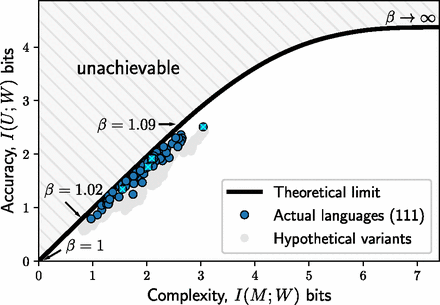
\includegraphics[width=0.7\linewidth]{efficient_colornaming_result}
        \caption{Different languages (blue circles) achieve near-optimal compression (IB curve in black)~\cite{zaslavsky:2018}. Reproduced with permission.}\label{efficient_colornaming_result}
    \end{figure}

    In \cref{efficient_colornaming_result}, it is possible to see evidence that languages efficiently compress ideas into words by optimising the tradeoff between complexity and accuracy of the lexicon according to the IB principle.

    This analysis corroborates the current theory on human language evolution. The drive for information-theoretic efficiency explains why human languages categorise colour as they do and may also apply to learning in general.

    Assuming the hypothesis, languages evolve to become more efficient in a tradeoff between conciseness (complexity, generalisation) and precision. The prediction capability is just an expected consequence of an efficient representation of meaning. The conciseness of the representation of knowledge, given an acceptable error margin, is a proxy of the agent's intelligence. The IB limit is an epistemic limit that is valid for machines, humans and aliens.

\section{Concluding Remarks}

<<<<<<< HEAD
- Cronologia X Didática
- Assumptions minhas. Finite
- Quantização
=======

>>>>>>> 1423702bbc26153edcfd7a58dee083e0fcfdf6ad



% \section{IB Learning}
% \subsection{The IB Lagrangian}

% \begin{itemize}
% 	\item IB solution assumes $P(X,Y)$ is given
% 	\item if unknown, MI intractable
% 	\item use proxies instead
% 	\item analitically solvable for distributions in the exponential family
% 	\item soft generalisation of minimal sufficiency
% \end{itemize}

% a task is a set of decisions to be taken given observed data;
% • a representation of a task is a function of data that can be computed and stored in memory for later acomplishment of the task.
% • an optimal representation is one that enables the best task performance given available data and resources.
% We need to differentiate 2 interwined but different representations in this discussion:
% 1. the representation of the training set (past data), stored in the weights of the network; 2. the representation of current input, encoded in the activations of the network;
% Each attend different tradeoffs (optimisation criteria):
% 1. weights need to store useful information for future decisions, without squandering resources in remembering spurious correlations or one-time events;
% 2. activations need to represent essential details of the scene at hand, without squandering resources in useless details;
% • Thedichotomyabovecreatesafundamentalproblem:desirablepropertiesoftheactivationsconcern representation of future data, while we only have past data to optimise a representation.
% • Information of what, for what, relative to what: Data reduces uncertainty in the task. The amount of uncertainty reduction is the information the data contains about the task. Reasoning about infor- mation requires specifying information of what (the data), for what (the task), relative to whatever prior uncertainty was present before the data was available.

% (Informationintheweights)Theyarguethatgivenasourcedata,andastochastictrainingalgorithm, the output weight w of the training process is a random variable (that depends on the stochasticity of the initialisation, training steps, and the data); i.e. w is a representation of the dataset D and we can talk about I(w;D). Instead of computing or optimising I(w;D), they want to control it by injecting noise in the weights that can be modulated between zero to an amount large enough that no information is left.